\documentclass{standalone} 

\usepackage{graphicx,tikz}
\usepackage{pgfplots,tikz-3dplot}
\pgfplotsset{compat=1.8}
\usetikzlibrary{shapes.geometric}
\usepgfplotslibrary{fillbetween}
\usetikzlibrary{patterns}

\begin{document}

	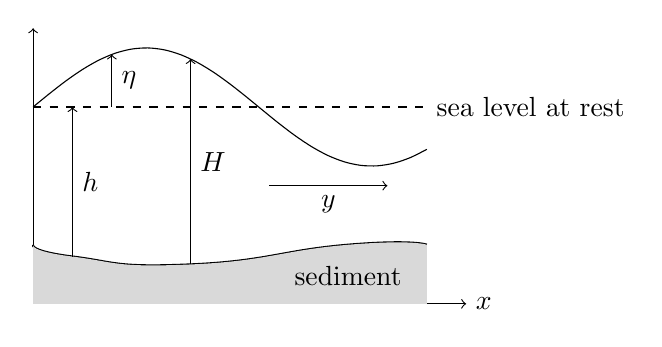
\begin{tikzpicture}
		% wave
		\def\wave{\x,{1+0.75*sin(20*pi*\x)}} 
		% coordinate system
		\draw[name path=xaxis] (0,-1.5) -- (5,-1.5);
		\draw[->] (0,-1.5) -- (5.5,-1.5) node[right] {$x$};
		\draw[->] (0,-1.5) -- (0,2);
		% draw wave
		\draw[name path=wave] plot[domain=0:5, smooth, variable=\x]  (\wave);
		% draw ground
		\draw[thick,-,name path=ground] plot [smooth,tension=1] coordinates { 
			(0,-0.75) (.5,-0.9) (2,-1) (4,-0.75) (5,-0.75)};
		% fill ground
		\tikzfillbetween[of=xaxis and ground]{gray!30};
		\node at (4,-1.15) {sediment};
		% fill wave
		%\tikzfillbetween[of=wave and ground]{cyan!30};
		% variables
		\draw[->] (1,1) -- (1,{1+0.75*sin(20*pi*1)}) 
			node[midway, right] {$\eta$};
		\draw[->] (2,-1) -- (2,{1+0.75*sin(20*pi*2)}) 
				node[midway, right] {$H$};
		\draw[->] (.5,-0.9) -- (0.5, 1)
				node[midway, right] {$h$};
		% sea level
		\draw[dashed] (0,1) -- (5,1) node[right] {sea level at rest};
		% velocity
		\draw[->] (3, 0) -- (4.5, 0) node[midway, below] {$y$};
	\end{tikzpicture}




\end{document}
